\documentclass[../main.tex]{subfiles}

\begin{document}
	\section{Statement of Cash Flows (Part 2)}
	
	The Statement of Cash Flows shows each major type of business activity that 
	caused a company’s cash to increase or decrease during the accounting  
	period. The major types of business activities are:
	\begin{itemize}[noitemsep]
		\item \textbf{Operating} - the cahs received and paid for day-to-day 
		activities with customers, suppliers and employees.
		\item \textbf{Investing} - The cash paid and received from buying and 
		selling long-term assets.
		\item \textbf{Financing} - The cash received and paid for exchanges 
		with lenders and stockholders. 
	\end{itemize}

	Preparing the Statement of Cash Flows involve five steps:
	\begin{enumerate}[noitemsep]
		\item Compute the net increase/decrease in Cash
		\item Compute and report net Cash provided or used in operating 
		activities.
		\item Compute and report net Cash provided or used in investing 
		activities.
		\item Compute and report net Cash provided or used in financing
		activities.
		\item Compute the net Cash flow by combining net Cash provided or used 
		in operating, investing, and financing activities and then prove it by 
		adding it to beginning Cash balance, and show that it equals to the 
		ending Cash balance. 
	\end{enumerate}

	\begin{figure}[ht]
		\centering
		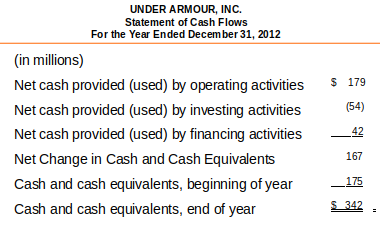
\includegraphics[width=0.7\columnwidth]{images/c11/cash_flows.png}
		\caption{\label{fig:soc_example} Statement of Cash Flows Example. 
		Notice three basic sections: operating activities, investing activities 
		and financing activities. This statement also includes a reconciliation 
		between beginning and ending Cash and Cash equivalents.}
	\end{figure}
	
	Although exceptions exist, a general rule is that operating cash flows 
	cause changes in Current Assets and Current Liabilities, investing cash 
	flows affect Noncurrent Assets, and financing cash flows affect Noncurrent 
	Liabilities or Stockholders’ Equity accounts
	
	\subsection{Operating Activities}
	
	The Operating Activities Section includes cash inflows and cash outflows 
	that result from the operations of the business and some incidental 
	business transactions i.e. Cash inflows and outflows that are directly 
	related to revenues and expenses.
	\begin{itemize}[noitemsep]
		\item Operating cash inflows include cash collected from customers,  
		receiving dividends, and receiving interest.
		\item Operating cash outflows include purchasing services and goods for 
		resale, paying salaries and wages, paying income taxes, paying interest.
	\end{itemize}

	\subsection{Investing Activities}
	
	The Investing Activities Section includes:
	\begin{itemize}[noitemsep]
		\item Cash inflows from the sale or disposal of equipment, and the sale 
		or maturity of investments in securities.
		\item Cash outflows for the purchase of equipment and the purchase of 
		investments in securities
	\end{itemize}
	The difference between these cash inflows and outflows is reported on the 
	statement of cash flows as a subtotal, \textbf{Net Cash Provided by (Used 
	for) Investing Activities.} Investing cash flows affect Noncurrent Assets.

	\subsection{Financing Activities}
	
	The financing activities section includes:
	\begin{itemize}[noitemsep]
		\item Cash inflows from borrowing from lenders through formal debt 
		contracts and issuing stock to owners
		\item Cash outflows for repaying principal to lenders, repurchasing 
		stock from owners, and paying cash dividends to owners.
	\end{itemize}
	The difference between these cash inflows and outflows is reported on the 
	Statement of Cash Flows as a subtotal, \textbf{Net Cash provided by (used 
	for) Financing Activities}. Financing cash flows affect Noncurrent 
	Liabilities or Shareholders’ Equity accounts.
	
	\subsection{Preparing Statement of Cash Flows}
	
	There are multiple methods to prepare the Statement of Cash Flows:
	
	\subsubsection{Analyzing the Cash Account}
	
	A company’s cash receipts and cash payments are recorded in the Cash 
	account in its general ledger. The Cash account is therefore a natural 
	place to look for information about cash flows from operating, investing, 
	and financing activities:
	
	\begin{figure}[ht]
		\centering
		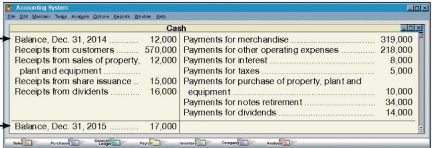
\includegraphics[width=1\columnwidth]{images/c11/cash_account_analysis.png}
		\caption{\label{fig:cash_account_analysis} Cash Account Analysis. 
		Individual cash transactions are summarized in this Cash account 
		according to the major types of cash receipts and cash payments. For 
		instance, only the total of cash receipts from all customers is listed. 
		Individual cash transactions underlying these totals can number in the 
		thousands. Accounting software is available to provide summarized cash 
		accounts.}
	\end{figure}
	
	Preparing a statement of cash flows from the Cash account above requires 
	determining whether an individual cash inflow or outflow is an operating, 
	investing, or financing activity, and then listing each by activity:
	\begin{figure}[ht]
		\centering
		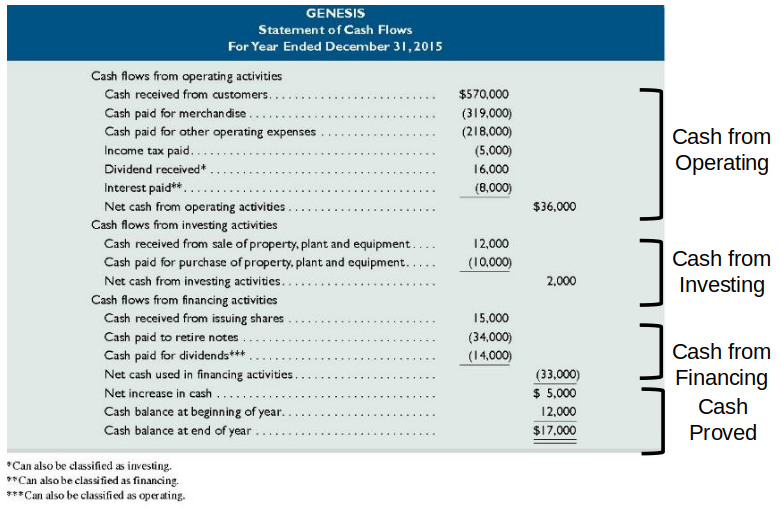
\includegraphics[width=1\columnwidth]{images/c11/from_cash_acc.png}
		\caption{\label{fig:from_cash_account} Statement of Cash Flows from 
		Cash Account}
	\end{figure}

	However, preparing the Statement of Cash Flows from an analysis of the 
	summarized Cash account has two limitations:
	\begin{itemize}[noitemsep]
		\item Most companies have many individual cash receipts and payments, 
		making it difficult to review them all. Accounting software minimizes 
		this burden, but it is still a task requiring professional judgment for 
		many transactions.
		\item The Cash account does not usually carry an adequate description 
		of each cash transaction, making assignment of all cash transactions 
		according to activity difficult.
	\end{itemize}
	
	\subsubsection{Analyzing Noncash Accounts}
	
	A second approach to preparing the statement of cash flows is analyzing 	
	noncash accounts. This approach uses the fact that when a company records 
	cash inflows and outflows with debits and credits to the Cash account, it 
	also records credits and debits in noncash accounts (reflecting 
	double-entry accounting). Many of these noncash accounts are Statement of 
	Financial Position accounts. For instance, from the sale of land for cash. 
	Others are revenue and expense accounts that are closed to equity. For 
	instance, the sale of services for cash yields a credit to Services Revenue 
	that is closed to Retained Earnings for a corporation. 
	
	In summary, all cash transactions eventually affect noncash statement of 
	financial position accounts. Thus, we can determine cash inflows and 
	outflows by analyzing changes in noncash statement of financial position 
	accounts i.e.
	
	\begin{equation}
		\text{Assets} = \text{Liabilities} + \text{Stockholders' Equity}
	\end{equation}
	\begin{equation}
		\text{Cash} + \text{Noncash Assets} = \text{Liabilities} + 
		\text{Stockholders' Equity}
	\end{equation}
	\begin{equation}
		\text{Cash} = \text{Liabilities} + 
		\text{Stockholders' Equity} - \text{Noncash Assets}
	\end{equation}
	\begin{equation}
		\Delta \text{Cash} = \Delta \text{Liabilities} + \text{Stockholders' 
		Equity} - \text{Noncash Assets}
	\end{equation}
	
	The derivation above shows that by analyzing noncash Statement of Financial 
	Position accounts and any related Income Statement accounts, we can prepare 
	a Statement of Cash Flows. To prepare a Statement of Cash flows by 
	analyzing the Income Statement and changes in Balance Sheet accounts, we 
	need the following information:
	\begin{itemize}[noitemsep]
		\item Comparative Balance Sheets for the beginning and end of the 
		period covered by the Statement of Cash Flows.
		\item An Income Statement for the period between the comparative 
		Balance Sheet dates.
		\item Additional details concerning selected accounts that increase and 
		decrease as a result of investing and/or financing activities.
		\item  Additional transactions that do not involve cash.
	\end{itemize}
	
	\subsection{Reporting Cash Flows}
	
	\subsubsection{Reporting Operating Cash Flows}
	
	Two alternative methods may be used when presenting the operating 
	activities section of the Statement of Cash Flows:
	\begin{itemize}[noitemsep]
		\item The direct method reports the total cash inflow or outflow from 
		each main type of transaction (that is, transactions with customers, 
		suppliers, employees, etc.). The difference between these cash inflows 
		and outflows equals the \textbf{net cash provided by (used for) 
		operating activities}. The direct method of presentation provides more 
		detailed information on each input into overall operating cash flows, 
		which allows analysts to conduct more detailed analyses.  The direct 
		method provides:
		\begin{itemize}[noitemsep]
			\item more detailed information. 
			\item prepared by adjusted accrual basis to cash basis
			\item Identifies each inflow and outflow relationships. An increase 
			in some activities, such as sales, generally leads to an increase 
			in cash inflows from customers and cash outflows to inventory 
			suppliers. However, an increase in sales activity only loosely 
			affects other cash outflows, such as interest paid on loans. 
			Knowing the detailed components of operating cash flows allows 
			analysts to more reliably predict a company’s future cash flows.
			\item Investing and financing sections for the two methods are 
			identical.
		\end{itemize}
		\item The \textbf{indirect method} starts with Net Income from the 
		Income Statement and adjusts it by eliminating the effects of items 
		that do not involve Cash (for example, Depreciation) and including 
		items that do have cash effects. Adjusting Net Income for these items 
		yields amount of net cash provided by (used for) operating activities. 
		Using the indirect method, analyses of operating cash flows are limited 
		to using just the overall \textbf{Net Cash Provided (Used for) 
		Operating Activities}.
	\end{itemize}
	The point to remember about these two methods is that they are simply 
	different ways to arrive at the same number. Net cash flows provided by 
	(used for) operating activities is always the same under the direct and 
	indirect methods. Also, the choice between the two methods affects only the 
	operating activities section of the Statement of Cash Flows, not the 
	investing and financing sections.
	
	\begin{figure}[ht]
		\centering
		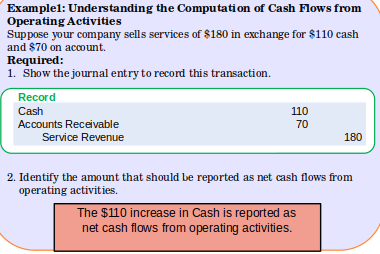
\includegraphics[width=0.9\columnwidth]{images/c11/cash_flows_eg1_p1.png}
		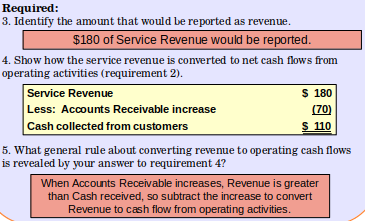
\includegraphics[width=0.85\columnwidth]{images/c11/cash_flows_eg1_p2.png}
	\end{figure}

	\begin{figure}[ht]
		\centering
		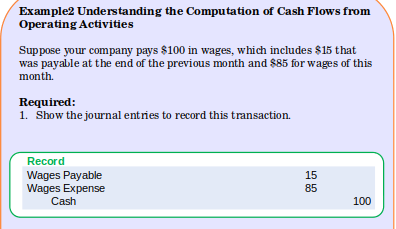
\includegraphics[width=0.9\columnwidth]{images/c11/cash_flows_eg2_p1.png}
		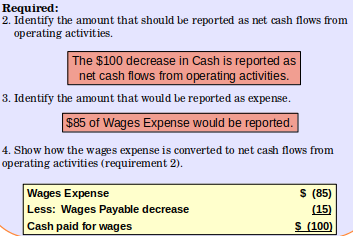
\includegraphics[width=0.85\columnwidth]{images/c11/cash_flows_eg2_p2.png}
		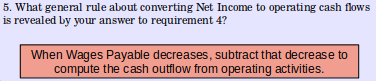
\includegraphics[width=0.85\columnwidth]{images/c11/cash_flows_eg2_p3.png}
	\end{figure}
	\begin{tabular}{|p{0.15\columnwidth}|p{0.35\columnwidth}|p{0.35\columnwidth}|}
		\hline
		& \textbf{Non-Cash Current Assets} & \textbf{Current Liabilities} \\
		\hline
		\textbf{Increase} & - Income Statement & + Income Statement \\ 
		\hline
		\textbf{Decrease} & + Income Statement & - Income Statement \\
		\hline
	\end{tabular}
	\begin{figure}[ht!]
		\centering
		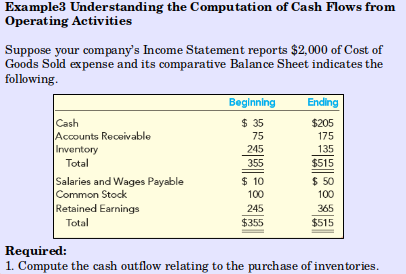
\includegraphics[width=0.95\columnwidth]{images/c11/cash_flows_eg3_p1.png}
		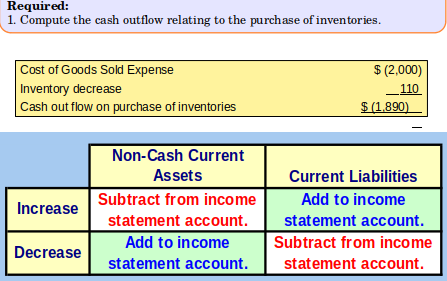
\includegraphics[width=0.95\columnwidth]{images/c11/cash_flows_eg3_p2.png}
		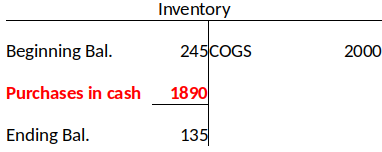
\includegraphics[width=0.60\columnwidth]{images/c11/cash_flow_eg3_p3.png}
		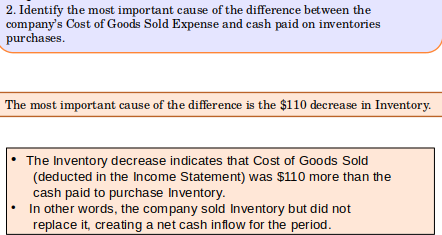
\includegraphics[width=0.95\columnwidth]{images/c11/cash_flows_eg3_p4.png}
		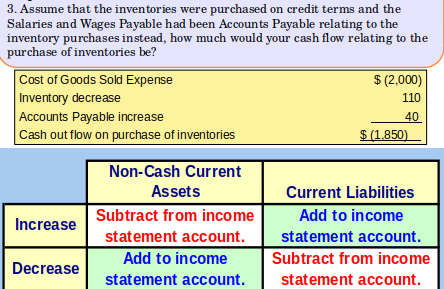
\includegraphics[width=0.95\columnwidth]{images/c11/cash_flows_eg3_p5.png}
		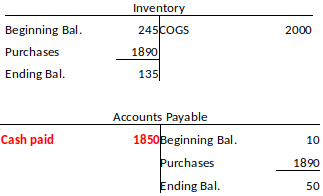
\includegraphics[width=0.75\columnwidth]{images/c11/cash_flows_eg3_p6.png}
	\end{figure}
	
	\begin{figure}[ht!]
		\centering
		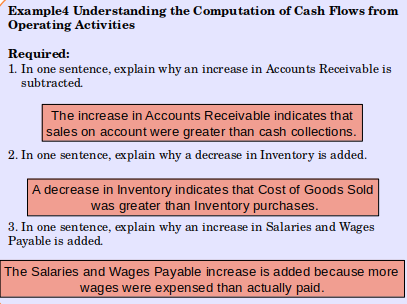
\includegraphics[width=0.9\columnwidth]{images/c11/cash_flows_eg4.png}
	\end{figure}

	This is an example of preparing a Statement of Cash Flows using the Direct 
	Method:
	\begin{figure}[ht!]
		\centering
		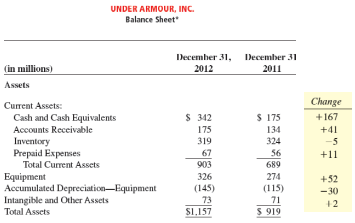
\includegraphics[width=1\columnwidth]{images/c11/ua_comparative_bs.png}
		\caption{Asset portion of Comparative Balance Sheet}
		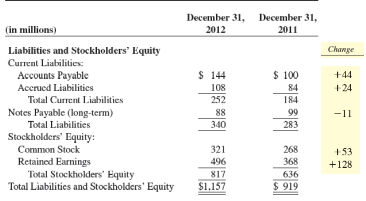
\includegraphics[width=1\columnwidth]{images/c11/ua_comparative_bs_liability_equity.png}
		\caption{Liability and Equity portion of Comparative Balance Sheet}
		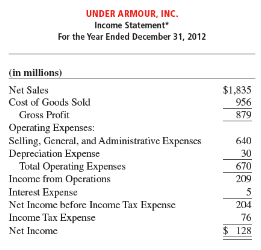
\includegraphics[width=0.65\columnwidth]{images/c11/ua_income_statement.png}
		\caption{Income Statement}
	\end{figure}
	
	With the direct method, we convert each revenue and expense on the Income 
	Statement to a cash flow. For example, since Accounts Receivable increased, 
	cash collections from customers were less than the amount of Sales Revenue 
	recorded in Accounts Receivable. So, we subtract the increase in 
	receivables from net sales to obtain the cash inflow.
	
\end{document}